% Yeah "slices" whatever lol
\documentclass{beamer}
\usepackage[style=authortitle-comp]{biblatex}
\usepackage[export]{adjustbox}

\title{Progress Report: Page Cache Consistency Model}
\author{Zhengyi Chen}
\date{\today}

\addbibresource{../main.bib}

\begin{document}
% Title page
\frame{\titlepage}

% Page -2
\begin{frame}
    \frametitle{
        Literature Review: (Shan, Tsai, \& Zhang. 2017\footcite{shan2017distributed})
    }
    \begin{itemize}
        \item {
            Concerns with the sharing of persistent memory --
            \begin{itemize}
                \item More or less similar to sharing regular memory, but\dots
                \item Data replication is key $\Rightarrow$ Multiple data provider.
            \end{itemize}
        }
        \item {
            Supports both Multi-Writer Multi-Reader and Multi-Writer Single-Writer Protocols
            \begin{itemize}
                \item MRMW ``support(s) great parallelism''
                \item MRSW enables ``stronger consistency''
            \end{itemize}
        }
        \item {
            Makes distinction between 3 variants of nodes:
            \begin{itemize}
                \item Commit Node -- Node who wishes to commit changes wrt. the system.
                \item Owner Node -- Node(s) who act as data provider for latest page content.
                \item Manager Node -- Node who provide (serialized) write access control to page.
            \end{itemize}
        }
    \end{itemize}
\end{frame}

\begin{frame}
    \frametitle{
        Literature Review: (Shan, Tsai, \& Zhang. 2017\footcite{shan2017distributed})
    }
    \begin{itemize}
        \item {
            For data replication and fault tolerance, necessitates:
            \begin{enumerate}
                \item Commit status logging (akin to journaled file system)
                \item Persistent Commit ID
                \item \textbf{Required} deg. of replication -- each ON shares to $N$ nodes.
            \end{enumerate}
        }
        \item {
            Fault tolerance is out of this thesis's scope. However\dots
            \begin{itemize}
                \item Prob. no need for requiring any degree of data replication.
                \item Dropping data replication req. $\Rightarrow$ no need for replication comms.
                \item Commit status logging \& persistent CID can be helpful \& should not introduce additional comms.
            \end{itemize}
        }
        \item {
            MRSW provides ``simpler and more efficient'' commits than MRMW -- no concurrent
            commits to same shared memory object exists.
            \begin{itemize}
                \item Also makes more sense from a CPU-accelerator dichotomy outlook (ofc. wrt. this thesis's system).
            \end{itemize}
        }
    \end{itemize}
\end{frame}

\begin{frame}
    \frametitle{MRSW: (Shan, Tsai, \& Zhang. 2017\footcite{shan2017distributed})}
    \begin{figure}
        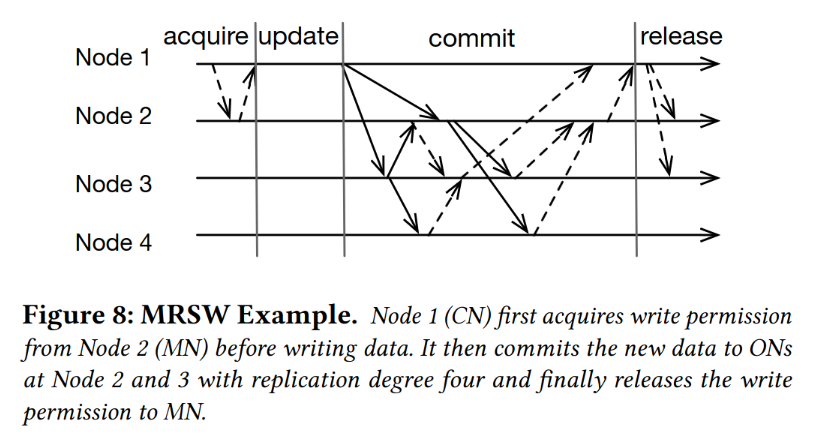
\includegraphics[width=\linewidth]{w12_slides_resources/dspm.fig8.png}
    \end{figure}
    Note: CN: Node 1, MN: Node 2, ON: Node 2 \& 3. Node 4 may or may not already
    share the committed page prior to acquire.
\end{frame}

% Page 0
\begin{frame}
    \frametitle{Literature Review: (Ramesh. 2023)}
    \begin{itemize}
        \item Popcorn-derived.
        \item {
            Sequential consistency, MRSW protocol offloaded onto sNIC:
            \begin{itemize}
                \item DSM protocol processor implemented on sNIC FPGA core.
                \item sNIC \textbf{keeps track of memory ownership, status, R/W permissions} at page level granularity.
                \item Removes the need for distinct memory management nodes.
                \item (i.e., the sNIC IS the memory management node -- except of course allocation).
            \end{itemize}
        }
        \item {
            Similar idea occurred in \textit{Concordia}\footcite{wang2021concordia}:
            \begin{itemize}
                \item Concurrency control and multicast offloaded to network switch.
                \item Authors claim this is more scalable (?)
            \end{itemize}
        }
    \end{itemize}
    \footnote{
        Ramesh., ``SNIC-DSM: SmartNIC based DSM Infrastructure for Heterogeneous-ISA Machines''
    }
\end{frame}

\begin{frame}
    \frametitle{Literature Review: (Endo, Sato, \& Taura. 2020)\footcite{EndoWataru2020MADD}}
    \begin{itemize}
        \item Eager Release Consistency.
        \item Prob. using MSI coherence protocol? Authors did not mention it.
        \item MRMW: use timestamps to store reader ``intervals''.
        \item {
            Introduces the home-migration concept:
            \begin{itemize}
                \item At commit, make the CN the home node instead of invalidating the home node.
                \item This removes communications needed for diff-merging at home node -- this can be done locally.
                \item No support for multiple home nodes.
            \end{itemize}
        }
        \item {
            No performance improvement over PGAS programming framework (OpenMPI).
        }
    \end{itemize}
\end{frame}

\begin{frame}
    \frametitle{Literature Review: (Endo, Sato, \& Taura. 2020)\footcite{EndoWataru2020MADD}}
    \begin{figure}
        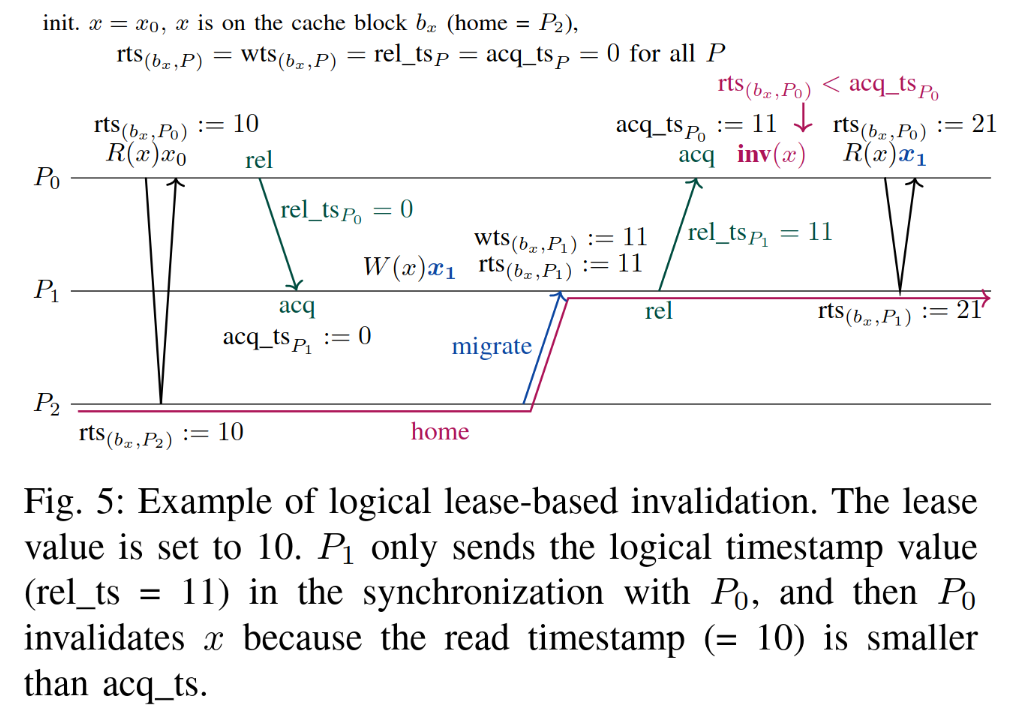
\includegraphics[width=\linewidth]{w12_slides_resources/menps.fig5.png}
    \end{figure}
\end{frame}

% Page 1
\begin{frame}
    \frametitle{The System}
    \begin{itemize}
        \item Remote node(s) abstracted as shared memory device ``\texttt{/dev/rshm}''
        \item {
            Heterogeneous Memory Management (HMM) ensures unified address space between
            local and device memory.
        }
        \item {
            Migration of pages between CPU and ``device'' is transparent to userspace
            -- no need for copying/mapping.
        }
        \item {
            In reality, ``\texttt{/dev/rshm}'' a handler for RDMA access between nodes.
            \begin{itemize}
                \item This involves remote read/write and moving page content between nodes.
                \item Local node serves as \emph{home node \& address space host} at share time.
                \item Remote nodes attached on \texttt{/dev/rshm} as accelerator.
            \end{itemize}
        }
    \end{itemize}
\end{frame}

% Page 2
\begin{frame}
    \frametitle{The Problem: Consistency Protocol}
    \begin{itemize}
        \item Single-Writer, Multiple-Reader Protocol
        % Why?
        % It may be that this mimics all sorts of logic for hardware acceleration
        % -- that is, in an HMM node each PCIe device have sole access to a page of memory.
        % For example, during machine learning you naturally can't access the same, say,
        % kernel by both CPU and GPU.
        % That said, I never shed a doubt on this issue except my advisor telling me not
        % to worry about it -- if I was asked this problem for some reason I'd be cooked!
        \item Need to be performant\dots with some ergonomics
        \item {
            Two Hypothetical Protocols:
            \begin{itemize}
                \item ``RwLock'' Consistency Protocol
                \item Acq-Rel Consistency Protocol
            \end{itemize}
        }
        \item {
            Former ensures \emph{strong} single-writer consistency
            \begin{itemize}
                \item -- Also easier to program with!
            \end{itemize}
        }
        \item Latter allows concurrent in-memory \emph{non-committal} computation
    \end{itemize}
\end{frame}

% Page 3
\begin{frame}
    \frametitle{``RwLock'' Consistency Protocol}
    Similar to a read-write lock where:
    \begin{itemize}
        \item Multiple readers can exist for a clean page -- the page is \textbf{shared}.
        \item Only one writer is allowed for a clean page -- the page becomes \textbf{exclusive}.
        \item {
            For one writer node be allowed sole write access to some page, all other
            readers need to have their page cache invalidated.
        }
        \item {
            While the sole writer node has not yet committed, no other reader or writer nodes
            are allowed to be served this page.
        }
        \item {
            When the sole writer commits, it becomes the new home node which serves the
            updated page content.
        }
        \item {
            Invalidates reader must fetch from MN for read access, which maintains RAW ordering.
        }
    \end{itemize}
\end{frame}

% Page 4
\begin{frame}
    \frametitle{``RwLock'' Consistency Protocol}
    \begin{figure}
        \centering
        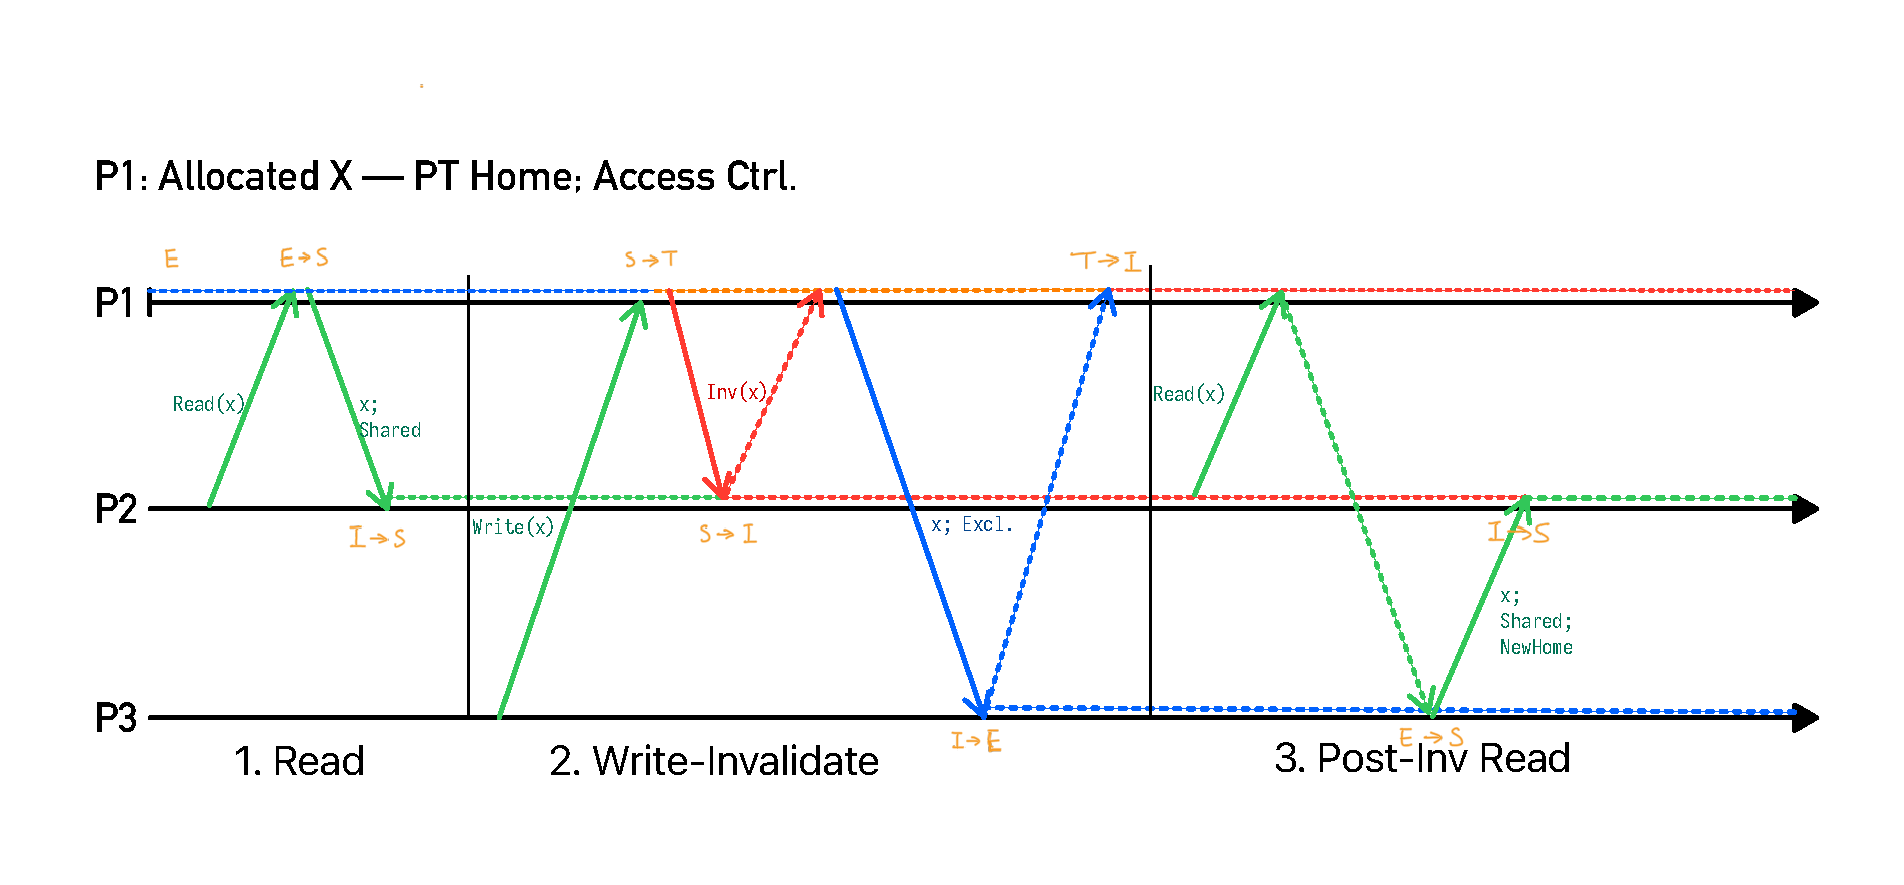
\includegraphics[width=\linewidth]{
            w12_slides_resources/Fig-RwlockProtocol 2023-12-06 19_05_06.pdf
        }
    \end{figure}
\end{frame}

% Page 5
\begin{frame}
    \frametitle{Acq-Rel Consistency Protocol}
    In RwLock's case, read requests result in installation of read-only pages at
    remote nodes.

    Alternatively, this protocol allows read/write pages to be installed at remote
    nodes at read time. Such writes are \emph{non-committal} and cannot be synced
    with the entire system.

    To summarize:
    \begin{itemize}
        \item {
            ``Readers'' can write to its locally installed page without any means
            to synchronize the change.
        }
        \item {
            ``Writers'' need to acquire global write access from the \emph{PT node},
            which invalidates all shared pages.
        }
        \item {
            i.e., Instead of write-invalidate, perform acquire-invalidate.
        }
    \end{itemize}

    This may require pages to be marked as CoW if the sharer wants also to act as a home node.
\end{frame}

% Page 6
\begin{frame}
    \frametitle{Consistency Protocol: Knobs and Mods}
    We can modify these two protocols further as follows:
    \begin{itemize}
        \item {
            Multi-home Protocol: instead of having one home at a time, have
            multiple homes (e.g., when writer commits) to prevent network bottleneck.
            \begin{itemize}
                \item Extra metadata can limit scalability (e.g., granularity of directories)
            \end{itemize}
        }
        \item {
            Auto-share: Automatically share pages at commit time using 1-way
            communications.
            \begin{itemize}
                \item Potential for communication reduction -- debatable.
            \end{itemize}
        }
        \item {
            Request aggregation: Aggregate RDMA requests for optimal RDMA transfer performance.
            \begin{itemize}
                \item Need to be coherent with program sequence!
            \end{itemize}
        }
    \end{itemize}
\end{frame}

\begin{frame}
    \frametitle{Why this design?}
    \begin{itemize}
        \item Largely inspired by DSPM\footcite{shan2017distributed}.
        \item Removed arrows for enforced data duplication -- duplication is solely on-demand.
        \item {
            Introduces transitional state ``T'':
            \begin{itemize}
                \item Used to flag a page as unserviceable -- visible only at MN.
                \item All read/write access to T-page is kept on hold until MN receives commit msg.
                \item After commit, MN forwards queued R/W access to moved home.
                \item This (at least) maintains RAW, WAW data dependency for whichever interleaving issues.
                \item Removing T allows stale data to be served -- violates RAW for better throughput.
            \end{itemize}
        }
        \item Extensible (as mentioned in prior page).
    \end{itemize}
\end{frame}

\begin{frame}
    \frametitle{Why not this design?}
    At the very least\dots
    \begin{itemize}
        \item {
            De-coupled home and access-management nodes require:
            \begin{itemize}
                \item Each home node need to be MN-aware (easy).
                \item {
                    MN need to be home-aware (also easy with single-writer, but spatial complexity is a concern):
                    \begin{itemize}
                        \item Naive directory scheme is not scalable.
                        \item Coarse directory scheme (e.g., SGI Origin 2000) is wasteful (but may be the fastest in practice).
                        \item Distributed directory scheme may provide terrible latency.
                        \item More sophisticated schemes are possible but needs work \& experimentation.
                    \end{itemize}
                }
            \end{itemize}
        }
        \item {
            Strict consistency limits throughput.
        }
    \end{itemize}
\end{frame}

% Page 7
\begin{frame}
    \frametitle{What about Consistency \textbf{Model}?}
    \begin{itemize}
        \item {
            The weaker a consistency model is, the more difficult it is to program with.
            \begin{itemize}
                \item {
                    Weak ordering architectures (e.g., ARMv8) more or less depends on
                    compiler/interpreter to emit barriers as see fit \footcite{Haynes_2022}.
                }
                \item {
                    Bad for usability/portability -- programs may need
                    to be compiled using a modified toolchain, else need to add these
                    synchronization instructions/function calls everywhere.
                }
            \end{itemize}
        }
        \item {
            \footcite{cai2018efficient} uses Partial Store Order.
            \begin{itemize}
                \item Preserves RAR, WAR -- ``synchronous read\dots asynchronous write''
                \item Easier to use than relaxed ordering.
            \end{itemize}
        }
        \item {
            \footcite{wang2021concordia} uses strong consistency, but warns about its scalability.
        }
    \end{itemize}
\end{frame}

% Page 8
\begin{frame}
    \frametitle{Consistency Model: Cont.}
    \begin{itemize}
        \item {
            Similar to Concordia\footcite{wang2021concordia}, the proposed protocols also assume
            strong consistency.
        }
        \item {
            Further work needed to see how to adapt these protocols for weaker consistency models.
            \begin{itemize}
                \item Low-hanging fruit: TSO
                \item Allowing read requests to be served for T-pages @ MN: W$\rightarrow$R violation.
                \item {
                    Allowing read requests to be served via non-MN homes: also W$\rightarrow$R violation
                    (exploits a race condition between write msg and invalidation msg).
                }
                \item Request workers work on one request at a time: no R$\rightarrow$W violation.
                \item W$\rightarrow$W violation simply cannot happen -- they always serialize @ MN.
            \end{itemize}
        }
    \end{itemize}
\end{frame}

\begin{frame}
    \frametitle{Summary}
    \begin{itemize}
        \item {
            Based on MSI coherence protocol, with possible T-state extension.
            \begin{itemize}
                \item T-state can be instead implemented as an additional flag parallel to MSI FSM.
                \item T-pages cannot be serviced by MN -- all read/write requests blocked.
            \end{itemize}
        }
        \item {
            One consistency model (for now): sequential consistency.
            \begin{itemize}
                \item Maintains RAW via T-state @ MN -- removing blocking on T-pages results in TSO.
                % Reads issued before Write -- read requests received before write.
                % Because RDMA QPs are FIFO, either read issued before or after write.
                % Assuming one worker thread works on requests sequentially, naturally WAR is preserved.
                % RAW is preserved because writes cannot be finished until commit message is received.
                % During which, T-state pages are blocked from being serviced.
                % This do introduce a semaphore-like situation, however...
                \item Maintains WAR via sequentially worked RDMA RQ.
                \item Maintains WAW via single-writer.
            \end{itemize}
        }
        \item {
            Two consistency protocols:
            \begin{itemize}
                \item RwLock consistency protocol only allows read-only sharing.
                \item {
                    Acq-Rel consistency protocol differentiates non-committal writes,
                    allows proc-local writable sharing.
                }
            \end{itemize}
        }
    \end{itemize}
\end{frame}
\end{document}